\newpage
\section{Gestion des signaux}

L'objectif de cette amélioration est de permettre l'envoi de signaux entre les différents threads, un signal étant traité dès que le thread l'ayant reçu a la main, et à condition qu'il ait un gestionnaire de signal, i.e. une fonction à exécuter lors de la détection d'un signal particulier. Outre l'intérêt de la communication entre différents threads, cette amélioration peut ensuite être utile pour la préemption par exemple dans le but d'indiquer au thread qu'il doit être préempté.

\subsection{Implémentation d'un signal}

\paragraph{}
Un signal dans l'implémentation choisie est un entier \texttt{int} ajouté à la structure thread initiale. Le champ des signaux couverts a été limité aux signaux POSIX. Les valeurs des signaux utilisés vont de 1 à 23 en x86, les différentes valeurs données pour d'autres architecture (comme ARM) sont également proches de cet interval. C'est pourquoi un entier est suffisant. Il sera ensuite manipulé à l'aide de masques. 

\paragraph{}
Les gestionnaires de signaux associé à un thread sont eux stockés dans un tableau de pointeurs de fonctions, également ajouté à la structure d'un thread.
Lorsqu'aucun gestionnaire n'est installé, le pointeur de fonction est alors \texttt{NULL}.

\paragraph{}
L'implémentation choisie est assez simple, et permet d'être proche de la signature de \texttt{signal} qui, bien que dépréciée, permet de gérer plus simplement la correspondance entre \texttt{p\_thread} et notre librairie.

\subsection{Envoi de signal et gestionnaire de réception}

\paragraph{}
Le gestionnaire de réception est une fonction choisie par l'utilisateur dans son programme. Elle sera appelée lors de la réception du signal par le thread. 

\paragraph{}
Deux fonctions principales ont donc été implémentées:
\begin{itemize}
\item La fonction \texttt{thread\_kill} équivalente à \texttt{pthread\_kill} qui permet d'envoyer un signal à un thread particulier. 
Dans le code proposé, le bit du signal reçu est positionné à 1 dans le champ de la structure thread.
\item La fonction \texttt{thread\_signal} correspondant à la fonction \texttt{signal} installe un gestionnaire de réception, pour un signal particulier, au thread courant.
Concrètement, il s'agit d'ajouter le pointeur de fonction de gestionnaire de signal au tableau des gestionnaires propre au thread.
\end{itemize}
Enfin, quand le thread destinataire prendra la main, il traitera le signal le plus prioritaire selon la règle suivante:\\
Les signaux SIGKILL et SIGSTOP ont la priorité absolue. Les autres sont classés dans l'ordre du numéro qui leur correspond selon la norme POSIX. Les signaux SIGUSER sont, par exception, les moins prioritaires et ne sont traités que si aucun autre signal n'a été reçu.

Le schéma \ref{signal} est proposé pour illustrer les actions effectués lors d'un échange de signaux.
\begin{figure}[!h]
  \caption{Envoi et réception de signal} %la légende
  \label{signal} 
  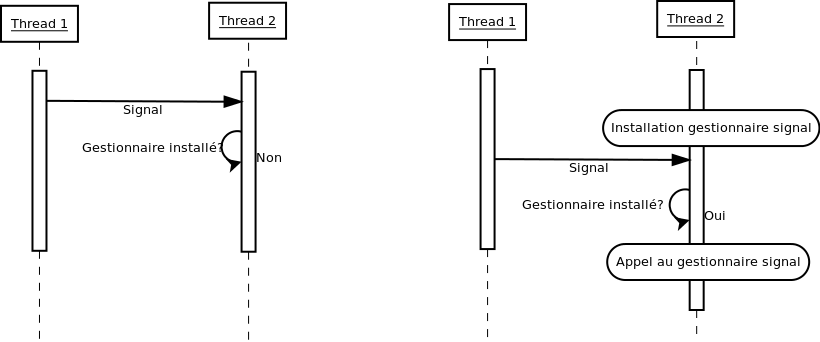
\includegraphics[scale=0.4]{signal.png}
\end{figure}


\subsection{Tests effectués}
Afin de tester cette nouvelle implémentation de signal, le programme \emph{07-signal-test} a été mis en place. 
\paragraph{Avec l'implémentation mise en place}
Le thread \texttt{main} crée tout d'abord un second thread qui va lui envoyer deux signaux successifs. Le gestionnaire n'étant pas installé, les signaux ne sont pas traités quand le thread \texttt{main} reprend la main. Puis, le gestionnaire de ces signaux est installé sur le \texttt{main} et le \texttt{main} créé un troisième thread lui renvoyant les deux signaux. Celui-ci traite le plus prioritaire comme prévu initialement. 

\paragraph{Avec pthread}
En relançant le test avec pthread, nous pouvons obtenir des résultats différents qui dépendent certainement du comportement de la fonction \texttt{signal}. Prenons par exemple, le résultat suivant :\\
> je suis le thread chef :: 0xb75436c0 \\
> je suis le thread 0xb7542358 et je vais envoyer le signal 4 à 0xb75436c0 \\
> je suis le thread 0xb75436c0 et je suis de retour dans le main \\
> je suis le thread 0xb7542358 et je vais envoyer le signal 8 à 0xb75436c0\\
> je suis le thread 0xb6d41358 et je vais envoyer le signal 4 à 0xb75436c0\\
> je suis vraiment le thread 0xb75436c0 et j'ai reçu le signal 8\\
> je suis le thread 0xb6d41358 et je vais envoyer le signal 8 à 0xb75436c0\\
> je suis vraiment le thread 0xb75436c0 et j'ai reçu le signal 8\\
> je suis vraiment le thread 0xb75436c0 et j'ai reçu le signal 4\\
> je suis vraiment le thread 0xb75436c0 et j'ai reçu le signal 4\\

Les signaux 4 et 8 sont traités. En effet, \texttt{pthread} traite tous les signaux reçus dans l'ordre des priorités. De plus, les deux premiers signaux non reçus avec notre implémentation sont également gérés. \\
En effet, les changements de contexte entre les deux threads sont ici plus fréquents. Ainsi, le thread est créé et est désordonnancé avant d'envoyer les signaux, ce qui permet au thread main d'installer le gestionnaire puis de redonner la main au thread qui va lui envoyer les signaux. \\
Le gestionnaire est donc toujours installé avant la réception des messages. Cependant, selon les lancements, la réception des derniers signaux diffère. Ici, le dernier signal 4 ne devrait pas être prise en compte. L'explication pourrait se trouver dans l'implémentation de la fonction \texttt{signal}, qui est dépréciée. 

\paragraph{Conclusion du test}
Ce test a le mérite de montrer que mélanger des signaux et du multithreading requiert une réflexion sur l'influence de l'ordonnancement sur le programme codé. Par ailleurs, il met en évidence les limites de la fonction \texttt{signal} à laquelle il faudrait préférer \texttt{sigaction}.%magnifique !

\subsection{Améliorations possibles}

\paragraph{}
A l'image de \texttt{p\_thread}, l'idée serait de traiter l'ensemble des signaux reçus dans l'ordre des priorités pour éviter une perte de l'information diffusée. Il faudrait donc appeler tous les gestionnaires de signaux reçus, pas seulement le prioritaire. La difficulté reposerait alors sur le comportement du programme si un thread traitant un signal se fait désordonnancer alors que le reste des signaux n'ont pas encore été traités.

\paragraph{}
Par ailleurs, les signaux SIGSTOP et SIGKILL ne doivent normalement pas admettre de gestionnaire. Cette amélioration peut être implémenté en imposant un gestionnaire par défaut à SIGKILL par exemple qui s'occuperait de tuer le thread courant. 

\paragraph{}
Enfin, dans le cas où notre programme aurait plusieurs threads noyaux, il pourrait être imaginé une communication hiérarchique par le biais de signaux uniquement possibles entre les threads noyaux, et d'autres entre les threads noyaux et utilisateur. De plus l'ordonnanceur pourrait alors se permettre lors de la réception d'un signal d'exéctuer le thread destinataire immédiatement.